\chapter{Future Work}

\section{Introduction}

This is clearly not the end of research on this method. While the groundwork has
been laid, there are plenty of avenues which need more study.

\section{Assumptions in the Analytical Approach}

In the analytical model presented here, the needle is assumed to be of zero
thickness, and yet an average temperature over an ellipse is taken which
represents the needle surface.  The model seems to work; however, there are
other ways to represent such a problem that may yield more accurate results. For
example, one may be able to approach the problem in terms of a needle with a
finite thickness, in which case the solution to the problem should be an
infinite series of Bessel functions in the isotropic case. One may be able to
tackle the problem from a finite-thickness needle approach for better results. In addition, a refined model could account for edge effects. \cite{axialerror}

\section{Extended Convergence Study}

While a convergence study for the numerical model was undertaken, it was relatively
informal, and executed for only one particular configuration of parameters. A
more thorough investigation of the convergence properties of the numerical model
should likely be undertaken, especially in light of the \(10\%\) error observed
in the convergence study done in this work.

\section{Improved Benchtop Method}

The benchtop apparatus was based on the use of glycerine and agar gels for
calibration. However, the current anisotropic benchtop method uses sugar and
salt. This makes the proper layering of the materials difficult. Moreover, the
device is limited to a tilt factor of \(30\) degrees from horizontal due to the
location of the bottle's opening. Presumably, this method could be improved upon
to allow for more accurate material layering and for an increased range of
needle angles.

In addition, the materials used only lend themselves to an anisotropy ratio of
87\%. There is plenty of room for improvement, in terms of suitable materials.
Figure \ref{fig:anisovmatl_rats} shows what material conductivity ratios are
required to achieve a given anisotropic conductivity ratio, assuming
equal-thickness layers. While salt and
sugar fare poorly, real-world materials have a wide range of conductivities
such that two materials with sufficiently different conductivities should be
possible to find.

\begin{figure}[h]
\centering
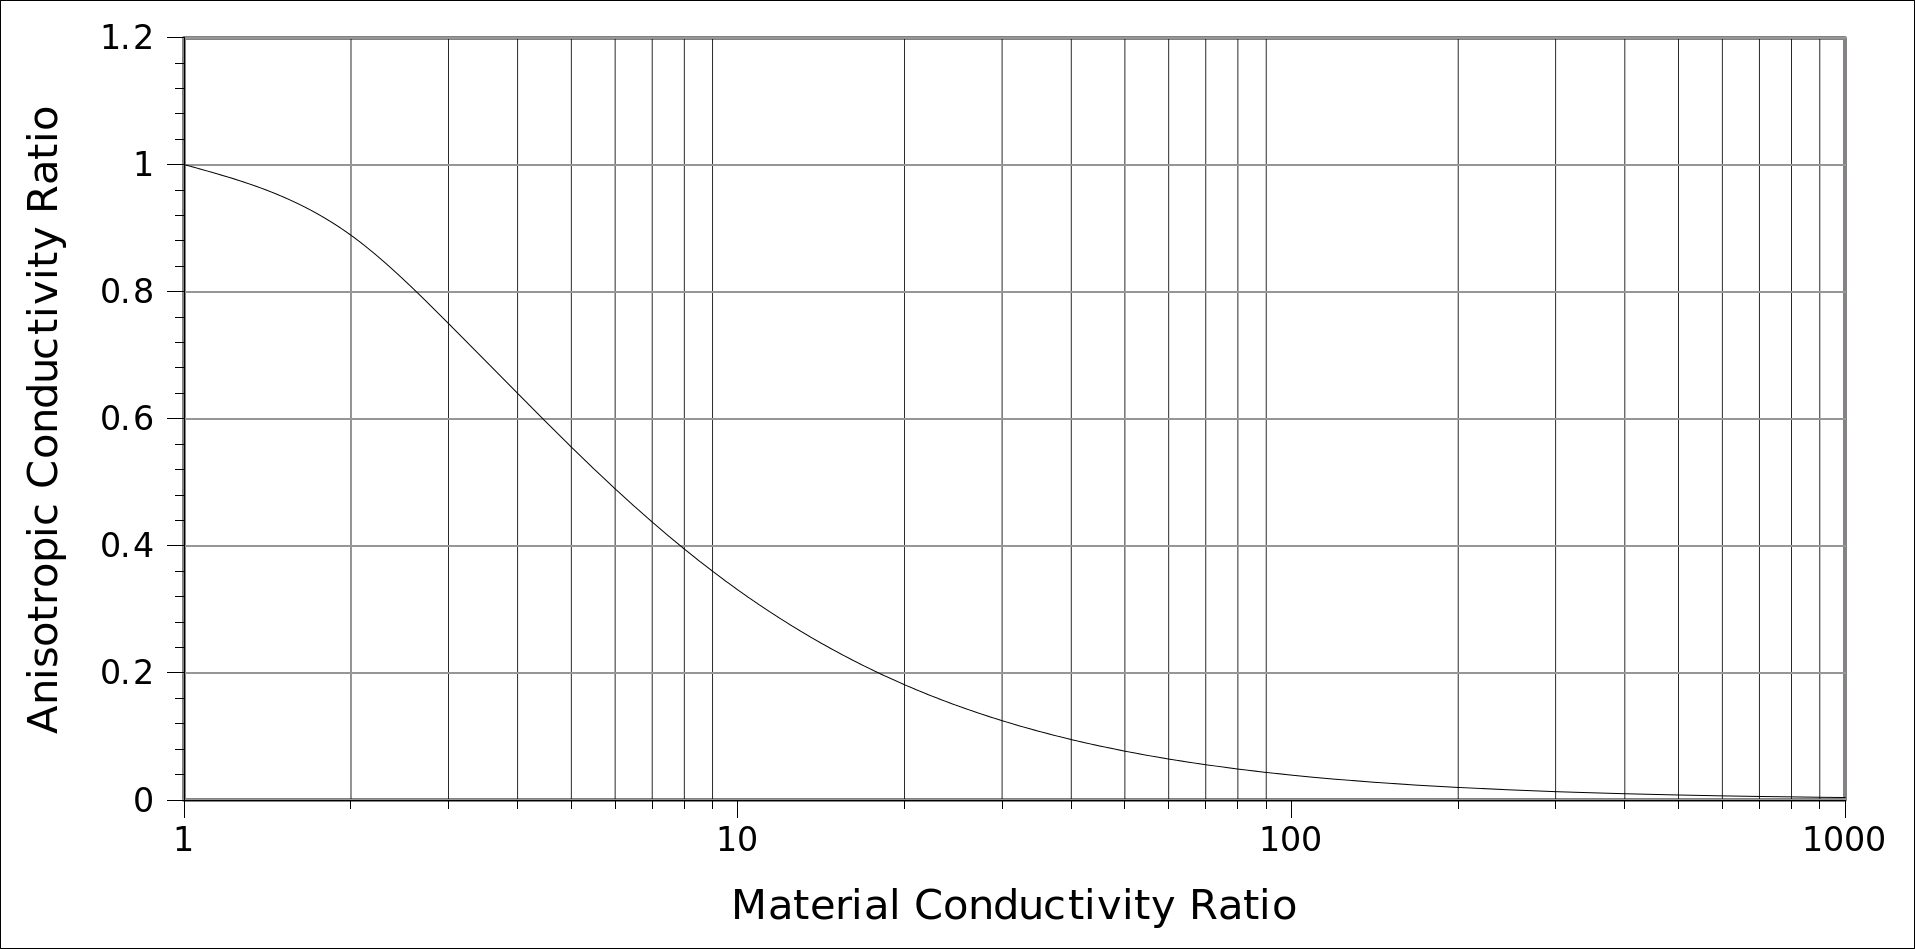
\includegraphics[width=0.7\textwidth]{fig/anisovmaterial_ratios.png}
\caption{Anisotropic Conductivity Ratio vs. Material Conductivity Ratio for the
layered geometry used in the benchtop experiments. It may take a very large
material conductivity ratio in order to achieve a relatively minor anisotropic
conductivity ratio.}
\label{fig:anisovmatl_rats}
\end{figure}

\section{Comprehensive Benchtop Measurements}

While enough benchtop measurements were taken to give a vague idea as to the
effectiveness of this measurement technique, there were not nearly enough
measurements to give a statistically valid conclusion regarding the slight
trend we were looking for. In addition to improving the benchtop method, there
need to be many more measurements taken, in order to draw statistically valid
conclusions.

\section{Comprehensive In-Situ Measurements}

The in-situ measurements presented in this document are very limited in scope.
One could easily spend much more time taking more measurements on more snow at
more angles, in order to better quantify the degrees of anisotropy in natural
snowpacks. More measurements would allow for a rigorous statistical analysis that
can show a trend with high confidence.


\section{Exploration of the Cooling Curve}

In the numerical and analytical models, the cooling curve is all but ignored. It
is believed that cooling curve models will yield analogous results, but this has
not been tested. Because of the importance of cooling curve measurements in the
real world (as they effectively double the number of measurements in a sample
and act as a consistency check on heating curve results),
verification of these expectations of analogous behavior should occur.

\section{A Method for Determining Anisotropic Thermal Conductivity From Measurements}

While this document lays the groundwork for determining anisotropic thermal
conductivity from measurements, a reliable method for converting measurements
into anisotropic thermal conductivities has not been found. This is, in part,
due to the discrepancy between the numerical and analytical approaches to
predicting effective thermal conductivity measurements as a function of angle
and degree of anisotropy, since the accuracy of either model is unknown.
Moreover, the lack of solid empirical data means that there is no evidence to
support either theory, outside of the isotropic case.

Given a reliable theory and data, one approach for ascertaining thermal
conductivity would be to find the degree of anisotropy for which the data as a
function of angle best fits the predicted \(k_{\textrm{eff}}\) curves
as a function of \(k_{xy}\) and \(k_z\). However, given the discrepancy in the
analytically-derived and numerically-derived theories, particularly in the
isotropic case, being able to do so with either theory doesn't seem valuable.

One possibility is that, instead of focusing on the measured conductivities as a
function of angle, that one should focus on the \emph{change} in measured
conductivities with respect to angle. This is because, while the actual predicted
values for \(k_{\textrm{eff}}\) disagree, the predicted percent difference
between two measurements may be less so, particularly for instances of smaller
anisotropy ratios. In fact, given low enough degrees of
anisotropy, it may be sufficient to compare linearizations of
\(k_{\textrm{eff}}\) vs. \(\theta\) curves. Only with more research can this
conjecture be shown to be valid.

One suggestion for collecting data to determine the correct theory is to take
measurements at the most extreme angles possible. In the case of measuring
conductivity at the center of the snowpack, \(45\) degrees from horizontal is
about the practical limit. However, tests conducted at the top of the snowpack
would be able to record measurements at \(90\) degrees from horizontal, the angle
at which the other expected extreme value is expected to occur. Given this data,
determining the correct theory may be easier. The author recommends, in addition
to other measurements, that this experiment is conducted in future research.
